\begin{wrapfigure}[11]{R}{0.42\textwidth}
%\begin{figure}[htb]
    \vspace{-10ex}
    \graphicspath{{./figures/}}
        \centering
        \subfloat[]{%
            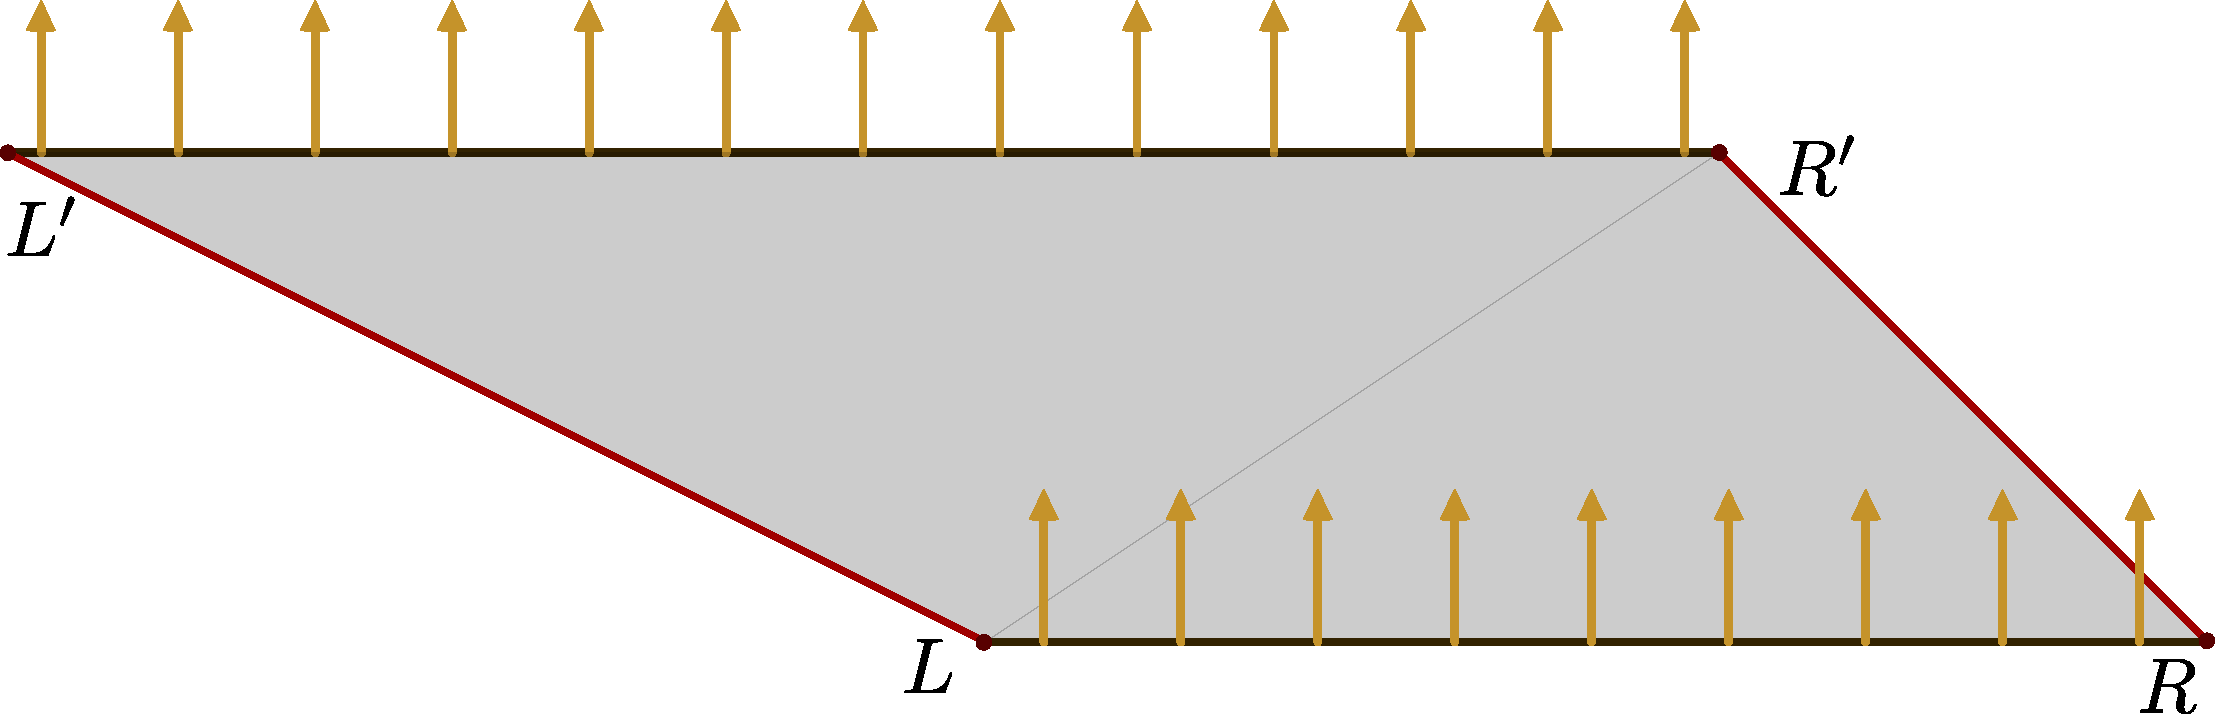
\includegraphics[width=0.25\textwidth]{figures/trapezoid.pdf}%
            \label{fig:segment_trapezoid}
        }%
        \hspace*{-0.25\textwidth}%
        \subfloat[\hspace*{-12em}]{%
            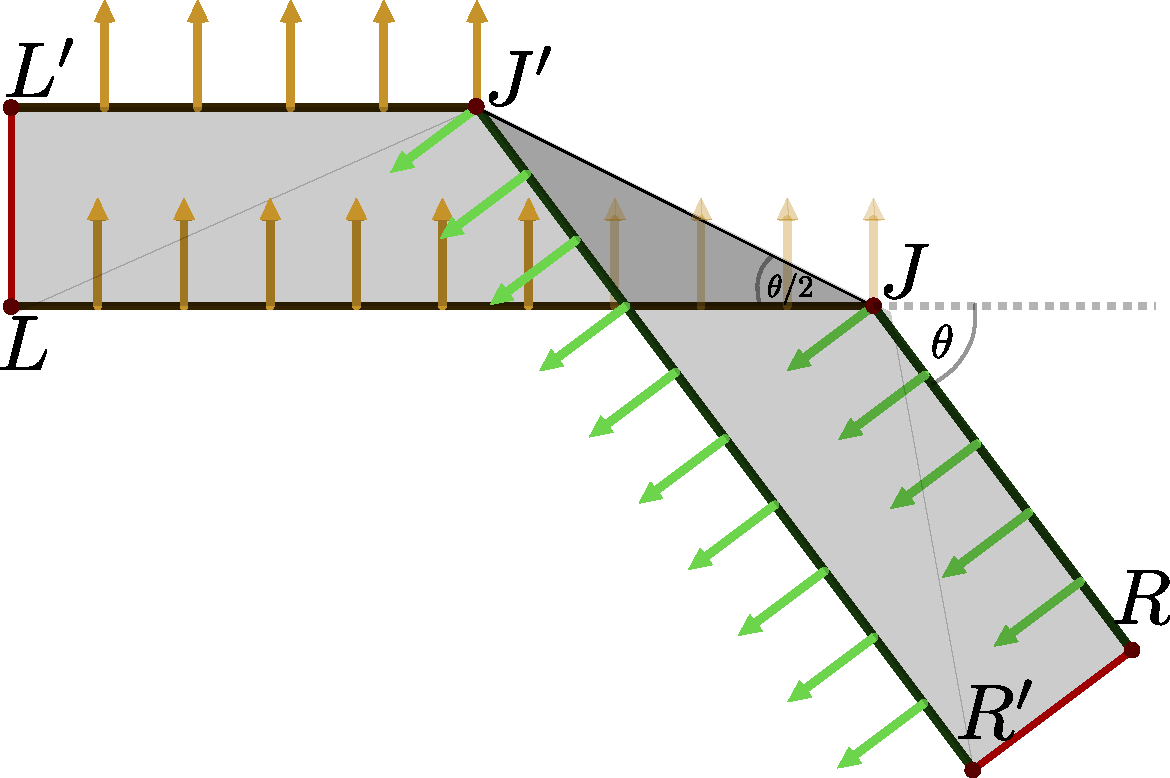
\includegraphics[width=0.4\textwidth]{figures/trapezoid_angles.pdf}%
            \label{fig:trapezoid_angles}
        }
        \caption{Trapezoid formed by evolving line segment (a), and the gluing of two adjacent trapezoids (b).}
        \label{fig:trapezoids}
%\end{figure}
\end{wrapfigure}
